\documentclass[11pt,aspectratio=169]{beamer}

\usepackage{amssymb}
\usepackage{physics}
\usepackage{enumerate}
\usepackage{mathtools}
\usepackage{amsmath}
% \DeclareMathOperator{\Tr}{Tr}

\title{Torus amplitudes and modular invariance}
\date[16.5.2022]{Seminar on Theoretical Physics}
\author{Otto T.P. Schmidt}
%\institute[Organizational Unit]{Organizational Unit\\can spread over 2 lines}
\institute[Department of Physics]{}
\usetheme{eth}

\colorlet{titlefgcolor}{ETHblue}
\colorlet{accentcolor}{ETHred}

\begin{document}

%\def\titlefigure{elements/title-page-image}		% Default image
%\def\titlefigure{elements/title-page-image-43}	% Use this for 4:3 presentations

\titleframe

% \colorlet{titlefgcolor}{ETHpurple}
% \def\titlefigure{elements/title-page-image-alt}
% \title{Different background}
% \titleframe

% \colorlet{titlefgcolor}{ETHgreen}
% \colorlet{titlebgcolor}{ETHgreen!60!black}
% \def\titlefigure{}
% \setlength{\titleboxwidth}{0.75\textwidth}			% Change box width
% \title{Or even a plain color, especially if your title is very long and leaves no space for what's behind the colored box}
% \titleframe

\tocframe

\section{Motivation}

\begin{frame}[fragile]{\underline{Interactions and observables}}

	In the study of string interactions, the ultimate goal will be the assignment of a probability for a certain process and the prediction of a physical cross section.
	\\~\\
	As outlined in Section 22, the computation of an observable cross section involves a series of steps:
	\begin{enumerate}
		\item Canonical representation of string diagram through moduli space
		\item Compute scattering amplitude by means of conformal field theory
		\item Convert scattering amplitude into a cross section
	\end{enumerate}
	
	
		




\end{frame}

\begin{frame}[fragile]{\underline{Loop amplitudes in string theory}}
	
	In order to obtain accurate scattering amplitudes of processes,
	one needs to include contributions from loops in string diagrams. 
	\\~\\
	These loops can be seen as contributions
	from the next higher order pertubation. 
	Graphically we consider the following processes:
	\begin{figure}[htbp]
		\centering
		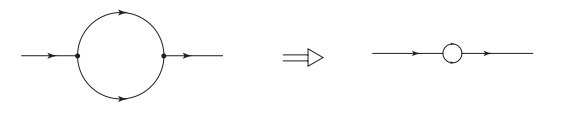
\includegraphics[width = 0.55\textwidth]{elements/Feynman loop}
	\end{figure}


\end{frame}

\begin{frame}{\underline{Ultraviolet divergence}}

	Amplitudes from virtual processes as depicted before can lead to ultraviolet (UV) divergences in quantum field theory (QFT).
	\\~\\
	Whereas QFT must employ complex renormalizations to deal with these UV divergences, we do not encounter these problems in string theory.
	
\end{frame}



\section{The moduli space of tori}

\subsection{One-loop open strings}

\begin{frame}[fragile]{\underline{One-loop open strings}}

	Before approaching the moduli space of tori, lets consider a one-loop open string with light-cone momentum $p^{+}$. This will serve as an intuitive analogon.

	The light-cone diagram is:
	\begin{figure}[htbp]
		\centering
		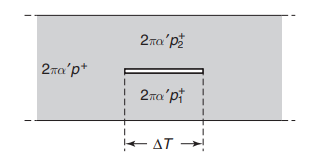
\includegraphics[width = 0.45\textwidth]{elements/one-loop open string.PNG}
	\end{figure}

	For fixed external momentum $p^+$ we find the two parameters: $\Delta T \in (0, \infty)$ and $p_{1}^{+} \in (0, p^+)$.
	\\
	$\rightarrow$ The class of Riemann surfaces of this process has two moduli.

\end{frame}

\begin{frame}{\underline{Canonical annulus}}

	Use $w = \tau + i \sigma$ and apply conformal transformations:
	\\~\\
	\begin{enumerate}
		\item Exponential map: $z = exp[\frac{w}{2 \alpha^{'} p^+}]$
		\item Linear fractional transformation: $\eta = \frac{1+iz}{1-iz}$
		% \item Canonical annulus: \textit{A region in} \mathbb{C} \textit{that is topologically an annulus can be mapped conformally to a canonical annulus}
		\item Canonical annulus: \textit{A region in $\mathbb{C}$ that is topologically an annulus can be mapped conformally to a canonical annulus}

	\end{enumerate}

	\begin{columns}
		\begin{column}{0.25\textwidth}
			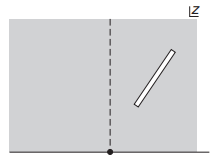
\includegraphics[width=\columnwidth]{elements/exponential map.PNG}
		\end{column}
		\begin{column}{0.25\textwidth}
			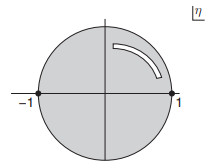
\includegraphics[width=\columnwidth]{elements/LFT.PNG}
		\end{column}
		\begin{column}{0.25\textwidth}
			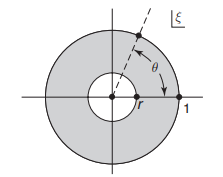
\includegraphics[width=\columnwidth]{elements/canonical annulus.PNG}
		\end{column}
	\end{columns}
	
\end{frame}

\subsection{Rectangular tori}

\begin{frame}{\underline{Rectangular tori}}

	In order to apply the concept of moduli spaces to a torus, we need to assure that a torus is indeed a Riemann surface.
	\\~\\
	Consider a rectangular region of $\mathbb{C}$. By applying the analytic identifications $z \sim z + L_1$ and $z \sim z + iL_2$
	we obtain a torus. This shows that the region remains a Riemann surface. 
	\\
	Graphically:
	\begin{columns}
		\begin{column}{0.25\textwidth}
			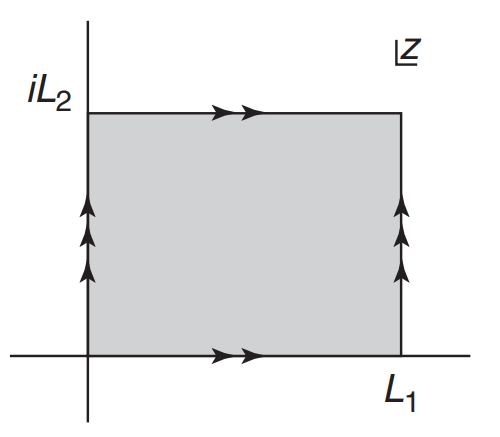
\includegraphics[width=\columnwidth]{elements/region C.PNG}
		\end{column}
		\begin{column}{0.2\textwidth}
			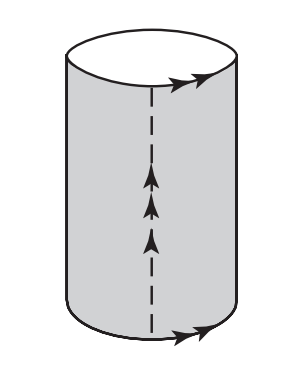
\includegraphics[width=\columnwidth]{elements/first ident.PNG}
		\end{column}
		\begin{column}{0.25\textwidth}
			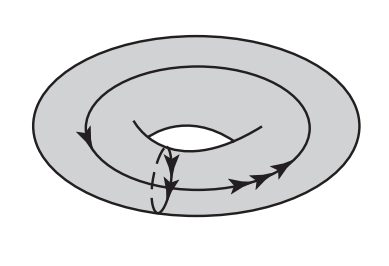
\includegraphics[width=\columnwidth]{elements/second ident.PNG}
		\end{column}
	\end{columns}


	
\end{frame}

\begin{frame}{\underline{Parametrisation}}

	We have:
	\\
	\begin{block}{Rectangular torus}
		$z \sim z + L_1$ and $z \sim z + iL_2$
	\end{block}
	\bigskip
	By applying $z' = \frac{z}{L_1}$ the identifications become:
	\begin{block}{Torus parameter T}
		$z' \sim z' + 1$ and $z' \sim z' + iT$ with $T = \frac{L_2}{L_1}$
	\end{block}

\end{frame}

\begin{frame}{\underline{Ultraviolet divergence}}

	T is a parameter of the torus but does not yet define the moduli space, i.e. tori with different T can be conformally equivalent.
	\\
	Consider the following series of conformal maps to a rectangular torus with $T<1$:

	\begin{figure}[htbp]
		\centering
		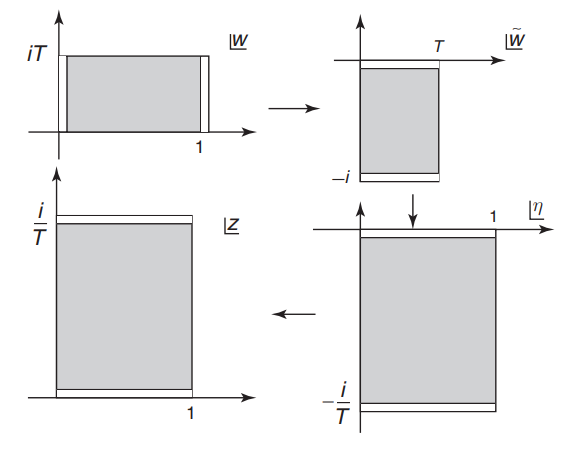
\includegraphics[width = 0.30\textwidth]{elements/three maps.PNG}
	\end{figure}
	\begin{block}{Rectangular torus}
		Tori with $T$ and $\frac{1}{T}$ are conformally equivalent
		\\
		$\rightarrow$ The moduli space can be chosen to be $T \in (0,1]$ or $T \in [1, \infty)$
	\end{block}
	
\end{frame}

\subsection{General tori}

\begin{frame}{\underline{General tori}}
	Rectangular tori represent only a subset of all conformally inequivalent tori. Let's construct a more general class of tori:
	\\
	\begin{block}{General construction of a torus as Riemann surface}
		Choose $\omega_1, \omega_2 \in \mathbb{C}$ with $\Im(\frac{\omega_1}{\omega_2}) > 0$.
		\\
		A torus is obtained by the indentifications $z \sim z + \omega_1$ and $z \sim z + \omega_2$.
		\\
		By scaling we obtain $z \sim z + 1$ and $z \sim z + \tau$ with $\tau = \frac{\omega_2}{\omega_1}$, $\Im(\tau) >0$.
	\end{block}
	$\rightarrow$ Note that for $\tau = iT$ ($\Leftrightarrow \Re(\tau) = 0$) we obtain the rectangular torus again.
	\begin{figure}[htbp]
		\centering
		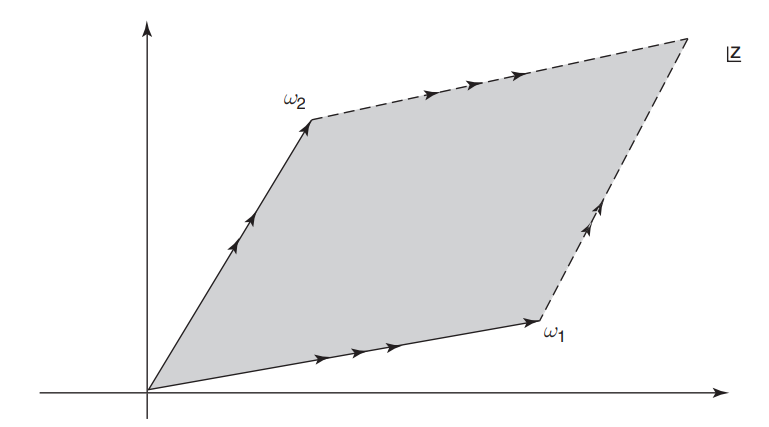
\includegraphics[width = 0.45\textwidth]{elements/general torus.PNG}
	\end{figure}
\end{frame}

\begin{frame}{\underline{Twisting the torus}}
	Intuitively, if a cylinder is twisted and the end surfaces are connected, we expect a different torus. 
	\\
	\underline{Formally}: Consider $\Re(\tau) \neq 0$ and a point $P = 0 \sim \tau$. We can reconstruct the rectangular $\textit{fundamental domain}$ by using the identification $z \sim z + 1$.
	\\
	\underline{Graphically}:
	\begin{figure}[htbp]
		\centering
		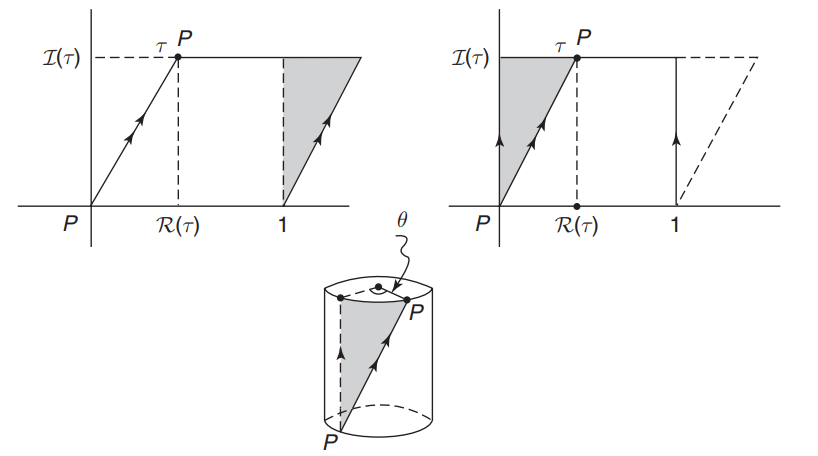
\includegraphics[width = 0.55\textwidth]{elements/twisted torus.PNG}
	\end{figure}
	
\end{frame}

\begin{frame}{\underline{Twisting parameter}}

	
	The point $P$ is no longer identified with a point on the perpendicular. Indeed the degree of twisting is parametrised by $\theta = 2\pi \Re(\tau)$.
	How does the twisting angle $\theta$ affect the torus parameter $\tau$?
	\\~\\
	Consider the map $\tau \rightarrow \tau + 1$:
	\begin{figure}[htbp]
		\centering
		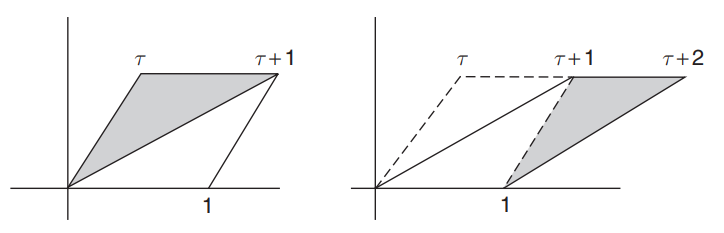
\includegraphics[width = 0.55\textwidth]{elements/tau map.PNG}
	\end{figure}
	With the identification $z \sim z + 1$ we can conclude $\tau \sim \tau + 1$ and hence $\theta \sim \theta + 2\pi$.
	\begin{block}{Note:}
		The "twisting" does not correspond to actual torsion. It is the mere identification of the points $P$.
	\end{block}
\end{frame}

\subsection{Fundamental domain}
\begin{frame}{\underline{Moduli space I}}
	So far we have established that $\Im(\tau) > 0 \Leftrightarrow \tau \in \mathbb{H}$.
	However, the identification $\tau \sim \tau + 1$ implies that the space of inequivalent tori is smaller. Indeed:
	\begin{block}{Strip $\mathcal{S}_{0}$}
		$\mathcal{S}_{0} = \{-\frac{1}{2} < \Re(\tau) \leq \frac{1}{2}, \Im(\tau) > 0\}$
	\end{block}
	Is $\mathcal{S}_{0}$ the moduli space of tori?
	\\
	For rectangular tori we found that $T$ and $\frac{1}{T}$ yield equivalent tori. Since $\tau = iT$ we have $\tau' = \frac{i}{T} = -\frac{1}{\tau}$.
	\begin{figure}[htbp]
		\centering
		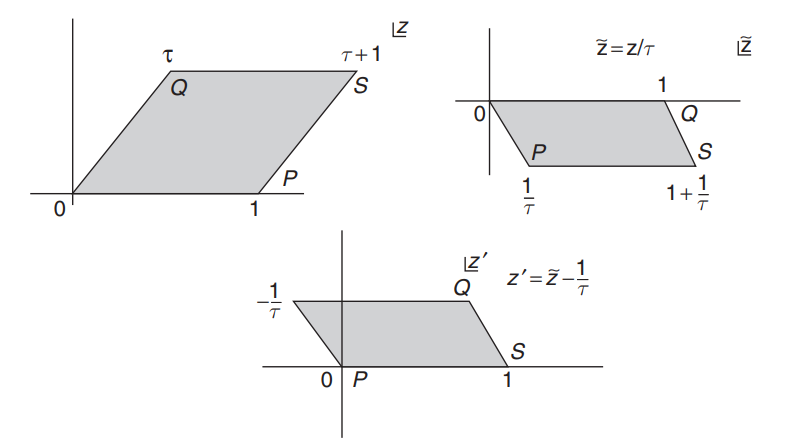
\includegraphics[width = 0.55\textwidth]{elements/s module trans.PNG}
	\end{figure}
\end{frame}

\begin{frame}{\underline{Moduli space II}}

	We have found two identifications with generators:
	\begin{block}{T-modular transform}
		$T\tau = \tau + 1$
	\end{block}
	\begin{block}{S-modular transform}
		$S\tau = -\frac{1}{\tau}$
	\end{block}
	The corresponding fundamental domain should be a subset of $\mathcal{S}_{0}$. Indeed, the S-modular transform identifies points in $|\tau| < 1$ with points in $|\tau| > 1$.
	\\
	Therefore we can postulate:
	\begin{block}{Fundamental domain $\mathcal{F}_{0}$}
		$\mathcal{F}_{0} = \{-\frac{1}{2} < \Re(\tau) \leq \frac{1}{2}, \Im(\tau) > 0, |\tau| \geq 1 \textrm{ and } \Re(\tau) \geq 0 \textrm{ if } |\tau| = 1\}$
	\end{block}
	
\end{frame}

\begin{frame}{\underline{Moduli space III}}

	Why is $\mathcal{S}_0$ not the correct moduli space?
	\\~\\
	Consider the torus $\tau = i$. Via the T-modular transform we have:
	\begin{equation}
		\tau_n = i + n \textrm{ for } n \geq 1
	\end{equation}
	Using the S-modular transform we get:
	\begin{equation}
		-\frac{1}{\tau_n} = -\frac{n}{n^2 + 1} + \frac{i}{n^2 + 1}
	\end{equation}
	These tori have $\Re(-\frac{1}{\tau_n}) \in [-\frac{1}{2}, 0]$ and $|-\frac{1}{\tau_n}| < 1$. 
	\\
	So they lie in $\mathcal{S}_0 - \mathcal{F}_0$.
	\\~\\
	$\rightarrow$ The complement of $\mathcal{F}_0$ in $\mathcal{S}_0$ therefore contains infinitely many copies of $\tau = i$. So we have to at least exclude this part of $\mathcal{S}_0$.
	
\end{frame}


\begin{frame}

	% \begin{columns}
	% 	\begin{column}{0.25\textwidth}
	% 		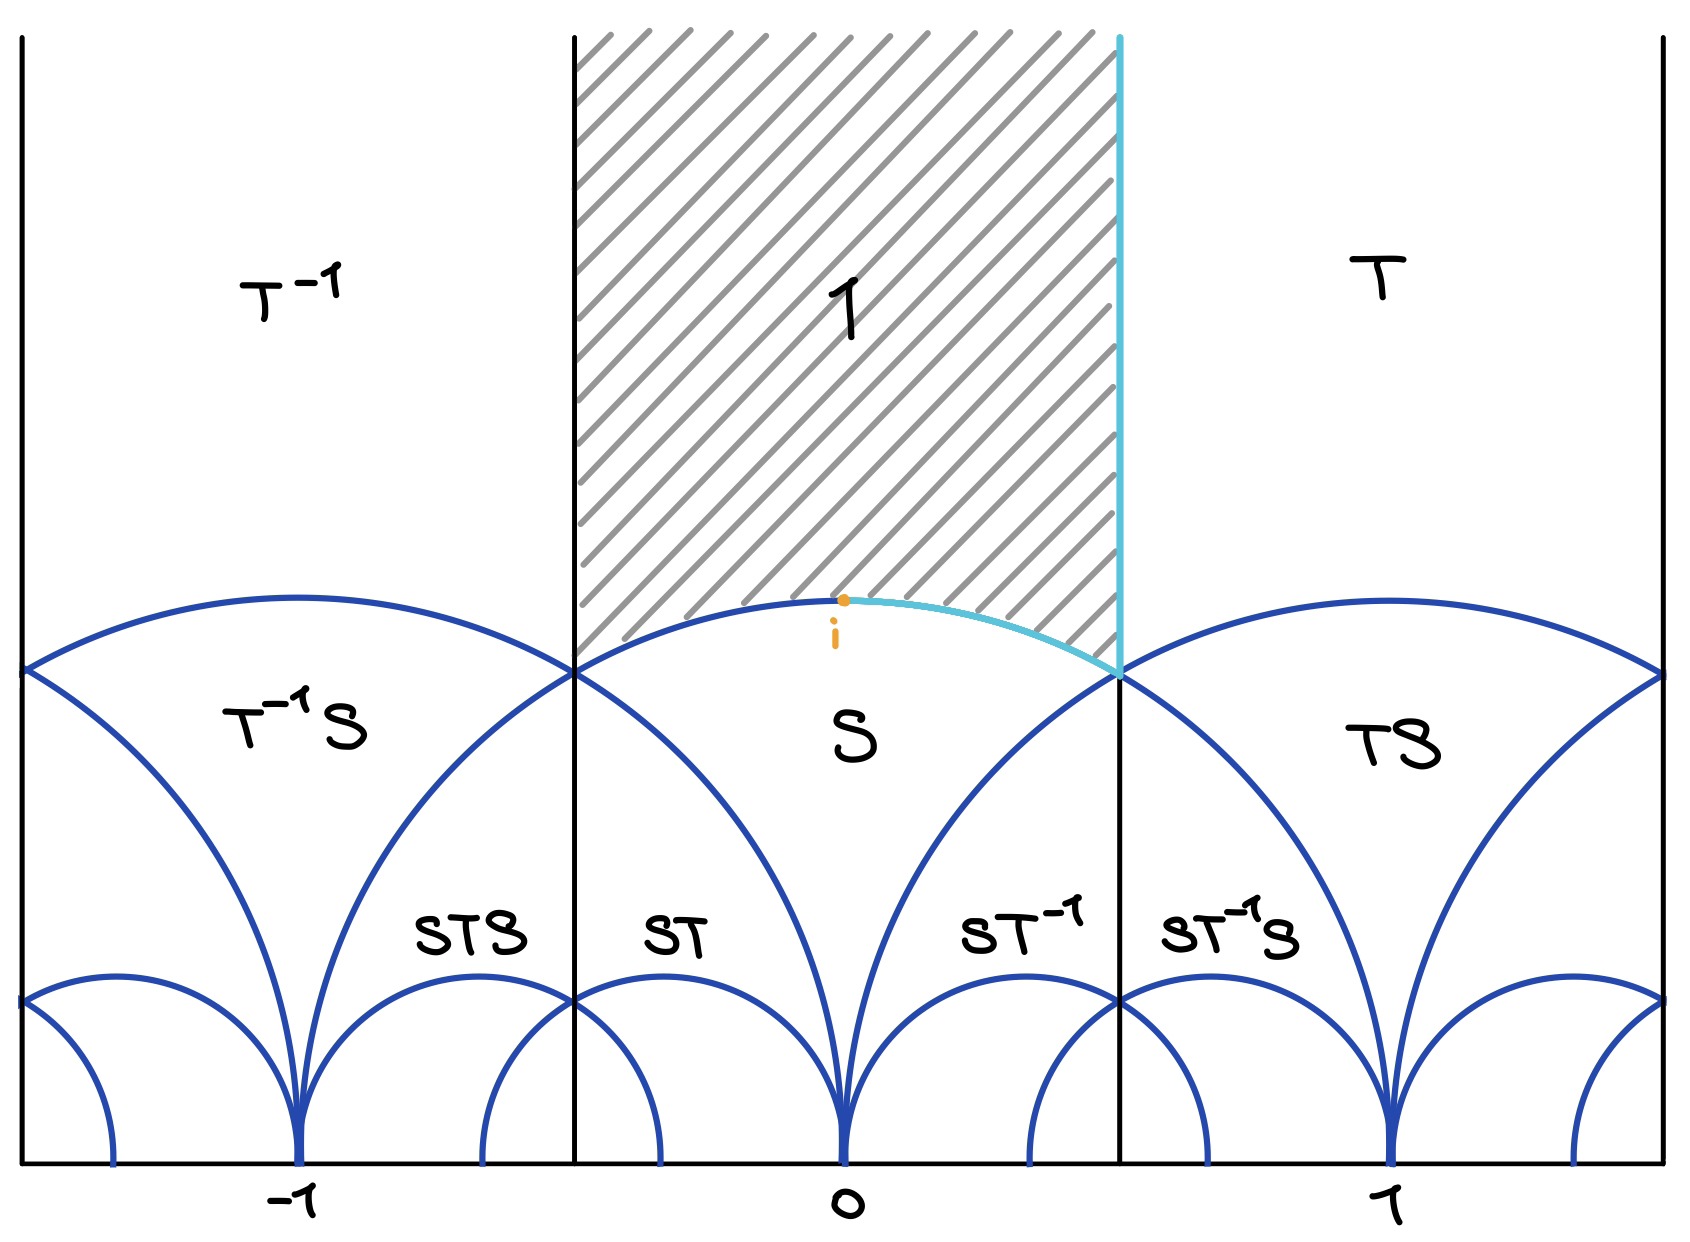
\includegraphics[width=\columnwidth]{elements/fundamental domain lucy.jpg}
	% 	\end{column}
	% 	\begin{column}{0.2\textwidth}
	% 		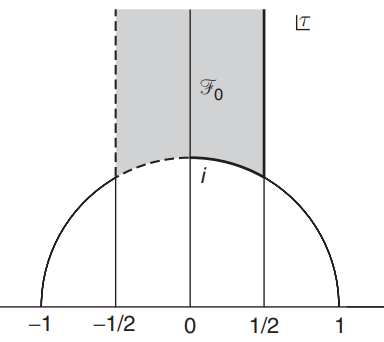
\includegraphics[width=\columnwidth]{elements/fundamental domain.PNG}
	% 	\end{column}
	% \end{columns}

	\begin{textblock*}{60mm}(0.05\paperwidth,0.25\paperheight)
		{\tiny \color{accentcolor}
		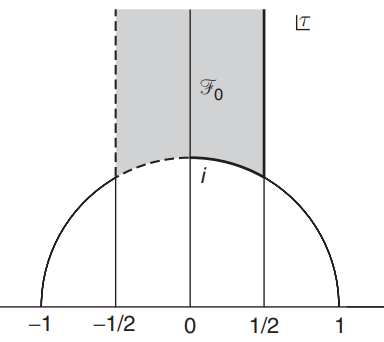
\includegraphics[width=60mm]{elements/fundamental domain.PNG}\\[2mm]
		}
	\end{textblock*}
	\begin{textblock*}{60mm}(0.45\paperwidth,0.32\paperheight)
		{\tiny \color{accentcolor}
		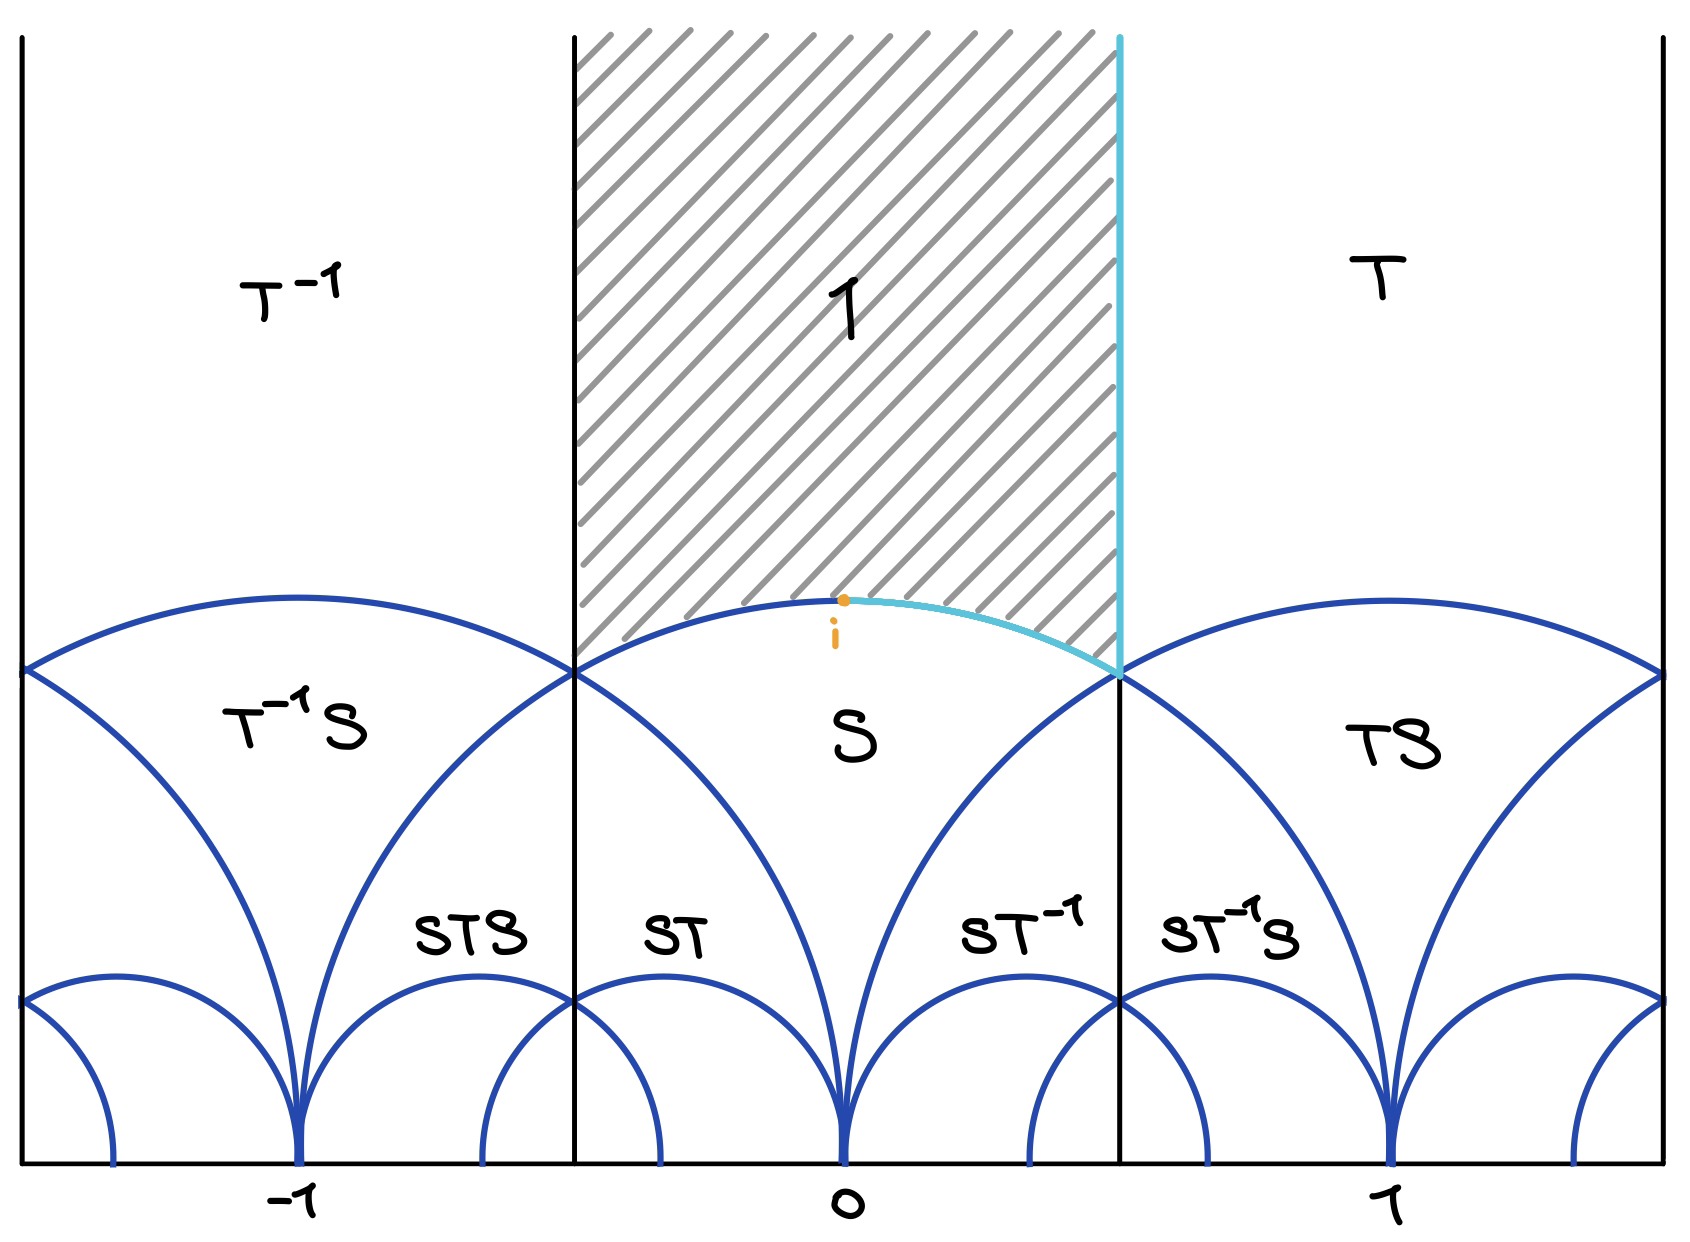
\includegraphics[width=60mm]{elements/fundamental domain lucy.jpg}\\[2mm]
		}
	\end{textblock*}

	
\end{frame}

\begin{frame}{\underline{Modular group $PSL(2, \mathbb{Z})$}}
	Consider a general linear fractional transformation $g \in G$:
	\begin{equation}
		g\tau = \frac{a\tau + b}{c\tau + d},~\Im(g\tau) = \frac{\Im(\tau)}{|c\tau + d|^2}
	\end{equation}
	with $a, b, c, d \in \mathbb{Z}$ and $ad- bc = 1$.
	\\
	Equivalently we can use a matrix representation:
	\begin{equation}
		[g] = \begin{pmatrix}
			a & b \\
			c & d \\
		\end{pmatrix},~\textrm{det}[g] = 1
	\end{equation}
	$\rightarrow$ $g$ satisfies the group homomorphism $\phi : G \rightarrow G$, $[g_1 g_2] \mapsto [g_1][g_2]$.
	\\
	We call $G$ the modular group $PSL(2, \mathbb{Z})$.
	\\~\\
	In matrix notation we see that $[T] = \big(\begin{smallmatrix}
		1 & 1\\
		0 & 1
	  \end{smallmatrix}\big)$ and $[S] = \big(\begin{smallmatrix}
		0 & -1\\
		1 & 0
	  \end{smallmatrix}\big)$ 
\end{frame}

\begin{frame}{\underline{Proving $\mathcal{F}_0$}}
	Let $G'$ be the set of projective transformations generated by T- and S-modular transforms.
	\\
	\begin{block}{Claim}
		For all $\tau \in \mathbb{H}$ exists $g \in G'$ such that $g\tau \in \mathcal{F}_0$
		\\
		$\rightarrow$ $\mathcal{F}_0$ contains exactly one copy of each inequivalent torus.
	\end{block}
	\underline{Step 1}: For each $\tau$ there is $g \in G'$ such that $\Im(g\tau)$ is largest.
	\\
	\underline{Step 2}: Show that $\tau' = T^{n}g\tau \in \mathcal{S}_0$ really is in $\bar{\mathcal{F}_0}$.
	\\
	\underline{Step 3}: Send $\tau \in \bar{\mathcal{F}_0}$ to $\tau \in \mathcal{F}_0$ via T- or S-transform.
\end{frame}

\section{Torus partition function}



\subsection{Single free boson in CFT}


\begin{frame}{\underline{Compactified bosonic string}}
	Consider one compactified dimension $X \sim X + 2\pi r$. In a free field theory the action can be written as 
	$S = \frac{1}{2\pi}\int \partial X \bar{\partial X}$.
	\\
	Intuitively we expect the partition function to count all states of the single free boson.
	\\~\\
	For a compactified closed string a Euclidean path integral yields the following expression for the partition function (using $q = e^{2\pi i \tau}$):
	\begin{equation}
		Z_r (\tau, \bar{\tau}) = \int e^{-S} = \frac{1}{|\eta|^2} \sum_{m, n} q^{\frac{1}{2}p_L^2}\bar{q}^{\frac{1}{2}p_R^2}
	\end{equation}
	where
	\begin{equation}
		p_L = \frac{m}{2r} + nr \textrm{ and }
		p_R = \frac{m}{2r} - nr
	\end{equation}
	and $p = \frac{m}{r}, w = nr$.
	% For such coordinates the boundary conditions read:
	% \begin{block}{BC}
	% 	$X_0(z + \tau, \bar{z + \tau}) = X_0(z, \bar{z}) + 2\pi r n'$ 
	% 	\\
	% 	and 
	% 	\\
	% 	$X_0(z + 1, \bar{z + 1}) = X_0(z, \bar{z}) + 2\pi r n$
	% \end{block}
	% The solution to the classical equations of motion reads:
	% \begin{equation}
	% 	X_0^{(n, n')}(z, \bar{z}) = \frac{2\pi r}{2i\tau_2}(n'(z - \bar{z}) + n(\tau\bar{z} - \bar{\tau}z))
	% \end{equation}
	% $\rightarrow$ one dimension is compactified

\end{frame}

\begin{frame}
	In order to understand this result we need to remember that the Hilbert space of the single free boson on a compactified world-sheet is in fact a product state:
	\begin{equation}
		\mathcal{H} = \mathcal{H}_{osc.} \otimes \bigoplus_{p, w} \mathcal{H}_{p, w}
	\end{equation}
	where $\mathcal{H}_{osc.}$ is the bosonic Fock space generated by the mode operators $\alpha_{-n}$ and $\bigoplus_{p, w} \mathcal{H}_{p, w}$ is the Hilbert space for different winding and momentum states.
	\\
	Let's denote the vectors as 
	\begin{equation}
		\ket{N,p} = \alpha_{-n_1} \dots \alpha_{-n_N} \ket{p} \textrm{ with } \sum n_i = N
	\end{equation}
	We can therefore expect:
	\begin{equation}
		Z = Z_{osc.} \times \sum_{p,w} Z_{p,w}
	\end{equation}
	\\
	So the partition function counts the oscillation modes of the string and the quantised momenta/winding.
\end{frame}

\begin{frame}{\underline{Dedekind eta function}}
	The $\textit{Dedekind eta function}$ is defined as:
	\begin{equation}
		\eta(\tau) = q^{\frac{1}{24}}\prod_{n=1}^{\infty}(1 - q^n)
	\end{equation}
	% Therefore we get:
	% \begin{equation}
	% 	(q\bar{q})^{-\frac{1}{24}}\Tr(q^{L_0}\bar{q}^{\bar{L_0}}) = \frac{1}{|\eta|^2}
	% \end{equation}
	\\~\\
	It is a modular form with weight $\frac{1}{2}$ and obeys:
	\begin{equation}
		\eta(\tau + 1) = e^{i\frac{\pi}{12}} \eta(\tau) \textrm{ and } \eta(-\frac{1}{\tau}) = \sqrt{-i\tau}\eta(\tau)
	\end{equation}
	
\end{frame}

\subsection{Modular invariance of partition function}

\begin{frame}{\underline{T-modular transform}}

	The partition function must remain invariant under a comformal transformation. Otherwise the inequivalent tori are not counted properly. 
	\\~\\
	Under a T-modular transform the partition function we obtained via a Euclidean path integral behaves like:
	\begin{align*}
		Z_r (\tau + 1, \bar{\tau} + 1) &= \frac{1}{|\eta|^2} \sum_{m, n} q^{\frac{1}{2}(\frac{m}{2r} + nr)^2}e^{2\pi i \frac{1}{2}(\frac{m}{2r} + nr)^2}
		\bar{q}^{\frac{1}{2}(\frac{m}{2r} - nr)^2}e^{-2\pi i \frac{1}{2}(\frac{m}{2r} - nr)^2} \\
		&= \frac{1}{|\eta|^2} \sum_{m, n} q^{\frac{1}{2}(\frac{m}{2r} + nr)^2}\bar{q}^{\frac{1}{2}(\frac{m}{2r} - nr)^2}e^{2 \pi i mn} \\
		&= Z_r (\tau, \bar{\tau}) \\
	\end{align*}

	
\end{frame}

\begin{frame}{\underline{S-modular transform}}
	To show modular invariance under a S-modular transform we need to make use of the Poisson resummation:
	\begin{block}{Poisson resummation}
		Let $f: \mathbb{R} \rightarrow \mathbb{C}$ be a Schwartz function $f \in \mathcal{S}(\mathbb{R})$.
		Then:
		\begin{equation}
			\sum_{n\in\mathbb{Z}} f(n) = \sum_{n\in\mathbb{Z}} \hat{f}(n)
		\end{equation}
	\end{block}
	We can write the partition function more aptly:
	\begin{equation}
		Z_r (\tau, \bar{\tau}) = \frac{1}{|\eta|^2} \sum_{p_L\in\Sigma, p_R\in\bar{\Sigma}} q^{\frac{1}{2}p_L^2}\bar{q}^{\frac{1}{2}p_R^2} = \frac{1}{|\eta|^2}\sum_{(p, w)\in\mathbb{Z}^2}e^{-\pi\begin{bmatrix} p \\ w \end{bmatrix}^T A \begin{bmatrix} p \\ w \end{bmatrix}}
	\end{equation}
	with 
	\begin{equation}
		A = -\begin{bmatrix} \frac{1}{2r^2}\tau_2 & i \tau_1 \\ i \tau_1 & 2r^2 \tau_2 \end{bmatrix}
	\end{equation}
	% The general case for the partition function reads:
	% \begin{equation}
	% 	\sum_{q\in \Sigma}e^{-\pi a q^2} = \frac{1}{a^{n/2}}\sum_{p\in \Sigma^*}e^{-\frac{\pi}{a}p^2}
	% \end{equation}
	% where $\Sigma$ denotes the $m, n$ lattice and $\Sigma^*$ the reciprocal lattice.
\end{frame}

\begin{frame}
	Using
	\begin{equation}
		\mathcal{F}(\exp{-\pi\begin{bmatrix} p \\ w \end{bmatrix}^T A \begin{bmatrix} p \\ w \end{bmatrix}}) = \det{A}^{-\frac{1}{2}}\exp{-\pi\begin{bmatrix} p \\ w \end{bmatrix}^T A^{-1} \begin{bmatrix} p \\ w \end{bmatrix}}
	\end{equation}
	\\
	or
	\begin{equation}
		\sum_{q\in \Sigma}e^{-\pi a q^2} = \frac{1}{a^{1/2}}\sum_{p\in \Sigma^*}e^{-\frac{\pi}{a}p^2}
	\end{equation}
	% We can write the partition function as:
	% \begin{align*}
	% 	Z_r (\tau, \bar{\tau}) &= \frac{1}{|\eta|^2} \sum_{p_L\in\Sigma, p_R\in\bar{\Sigma}} q^{\frac{1}{2}p_L^2}\bar{q}^{\frac{1}{2}p_R^2} \\
	% 	&= \frac{1}{|\eta|^2} \sum_{p_L\in\Sigma, p_R\in\bar{\Sigma}} e^{-\pi(-i\tau)p_L^2} e^{-\pi(i\bar{\tau})p_R^2} \\
	% \end{align*}
	we see that under the S-modular transform the partition function becomes (assuming $\Sigma = \Sigma^*$):
	\begin{align*}
		Z_r (-\frac{1}{\tau}, -\frac{1}{\bar{\tau}}) &= \frac{1}{|\tau||\eta|^2} \sum_{p_L\in\Sigma}e^{-\pi(\frac{1}{-i\tau})p_L^2}\sum_{p_R\in\bar{\Sigma}}e^{-\pi(\frac{1}{i\bar{\tau}})p_R^2} \\
		&= \frac{1}{|\tau||\eta|^2} \sum_{p_L\in\Sigma^*} \sqrt{-i\tau} e^{i\pi\tau p_L^2} \sum_{p_R\in\bar{\Sigma}^*} \sqrt{i\bar{\tau}} e^{-i\pi\bar{\tau}p_R^2} \\
		&= \frac{1}{|\tau||\eta|^2} |\tau| \sum_{p_L\in\Sigma, p_R\in\bar{\Sigma}} q^{\frac{1}{2}p_L^2}\bar{q}^{\frac{1}{2}p_R^2} \\
		&= Z_r (\tau, \bar{\tau})
	\end{align*}
\end{frame}

\begin{frame}{\underline{T-duality}}
	Consider again the momentum and winding for the compactified string:
	\begin{equation}
		p = \frac{m}{r} \textrm{ and } w = nr
	\end{equation}
	Let's interchange $p \rightarrow w$. 
	\\
	So:
	\begin{align*}
		p_L' &= \frac{w}{2} + p = \frac{n}{2r} + mr = p_L\\
		p_R' &= \frac{w}{2} + p = \frac{n}{2r} - mr = p_R \\
	\end{align*}
	This change however leaves the partition function invariant. We can conclude T-duality for the compactified closed string partition function:
	\begin{equation}
		Z_r (\tau, \bar{\tau}) = Z_{\frac{1}{2r}} (\tau, \bar{\tau})
	\end{equation}
\end{frame}

\begin{frame}{\underline{Return to flat space}}
	For $r \rightarrow \infty$ we get continuous momenta $p_L = p_R = \frac{m}{2r}$. 
	The contribution from winding $w = nr$ leads to a fast oscillating factor and hence vanishes.
	\\
	With $q = e^{2\pi i \tau}$ we can transform back to flat space:
	\begin{align*}
		Z(r) &= \frac{1}{|\eta|^2} \int_{-\infty}^{\infty}dk q^{\frac{1}{2}k^2}\bar{q}^{\frac{1}{2}k^2} \\
		&= \frac{1}{|\eta|^2} \int_{-\infty}^{\infty}dk e^{2\pi i \frac{1}{2}k^2 \tau}e^{-2\pi i \frac{1}{2}k^2 \bar{\tau}} \\
		&= \frac{1}{|\eta|^2} \int_{-\infty}^{\infty}dk e^{2\pi i \frac{1}{2}k^2 2 i \Im{\tau}} \\
		&= \frac{1}{|\eta|^2} \int_{-\infty}^{\infty}dk e^{-2\pi k^2 \Im{\tau}} \\
		&\propto \frac{1}{|\eta|^2} \frac{1}{\Im(\tau)^{\frac{1}{2}}}
	\end{align*}
	
\end{frame}









\subsection{Partition function via state trace}

\begin{frame}{\underline{Partition function via state trace}}
	A alternative approach to obtain the partition function is the state trace.
	\\~\\
	In quantum statistics:
	\begin{equation}
		Z = \Tr(e^{-\beta H}) \propto \sum_{\Phi}\bra{\Phi} e^{-\beta H} \ket{\Phi}
	\end{equation}
	The trace should run over all states of the torus. This means we need to find a propagator 
	which propagates through all state configurations of the torus.
	% \\~\\
	% Consider the state trace for a harmonic oscillator with number operators $N_L,N_R$ in 24 transverse dimensions:
	% \begin{equation}
	% 	\Tr(\bar{q}^{N_L - 1}q^{N_R - 1}) = (q\bar{q})^{-1}\prod_{n=1}^{\infty}(1 - \bar{q}^n)^{-24}(1 - q^n)^{-24} = \frac{1}{|\eta(\tau)|^{48}}
	% \end{equation}
	% Lets postulate:
	% \begin{equation}
	% 	Z(\tau) \propto \Tr(q^{L_0}\bar{q}^{\bar{L_0}})
	% \end{equation} 
	% with $q = e^{2\pi i \tau}$ and $L_0 = \sum \alpha_{-m}\alpha_m + \frac{1}{2}p_L^2$.
	

\end{frame}

\begin{frame}
 	The partition function can be split up into a part corresponding to the oscillation modes of the world-sheet string and the momentum.
	\\~\\
	The momentum states are counted via:
	\begin{equation}
		\sum_{p_L\in\Sigma, p_R\in\bar{\Sigma}} q^{\frac{1}{2}p_L^2}\bar{q}^{\frac{1}{2}p_R^2}  \xrightarrow{\text{$r \rightarrow \infty$}} \int_{-\infty}^{\infty}dk q^{\frac{1}{2}k^2}\bar{q}^{\frac{1}{2}k^2} \propto \frac{1}{\Im(\tau)^{\frac{1}{2}}}
	\end{equation}	
	A possible way of counting the oscillation states is:
	\begin{equation}
		\sum_{\Phi} \bra{\Phi} e^{2\pi i \tau L_0}e^{-2\pi i \bar{\tau} \bar{L}_0} \ket{\Phi} = \Tr(q^{L_0}\bar{q}^{L_0})
	\end{equation}
\end{frame}

\begin{frame}
	Is this a reasonable result? Two hints:
	\\~\\
	I:
	\begin{equation}
		\Tr(q^{L_0}) \propto \Tr(q^{\sum_{n=1}^{\infty}\alpha_{-n}\alpha_n}) = \prod_{n=1}^{\infty}(1 + q^n + q^{2n} + \dots) = \prod_{n=1}^{\infty}\frac{1}{1-q^n}	
	\end{equation}
	This is the partition function of a boson from the Bose-Einstein distribution.
	\\
	And:
	\begin{equation}
		\Tr(q^{L_0 - \frac{c}{24}}) = q^{-\frac{1}{24}} \prod_{n=1}^{\infty}\frac{1}{1-q^n}	= \frac{1}{\eta(\tau)}
	\end{equation}
	\\~\\
	II:
	\begin{align*}
		q^{L_0}\bar{q}^{\bar{L_0}} &= e^{2\pi i (\tau_1 + i \tau_2)L_0}e^{-2\pi i (\tau_1 - i \tau_2)\bar{L_0}}\\
		&= e^{2 \pi i \tau_1 (L_0 - \bar{L_0})}e^{-2\pi \tau_2 (L_0 + \bar{L_0})}
	\end{align*}
	We can interpret $L_0 - \bar{L_0}$ as the momentum $P$ which generates translation in $\sigma$. Similarly $L_0 + \bar{L_0}$ can be seen as Hamiltonian $H$ which generates $\tau$ translation.
	\\
	The propagator has then the interpretation of a $\tau$ and $\sigma$ sweep.

\end{frame}

% \begin{frame}{\underline{Hamiltonian interpretation}}
% 	In light-cone gauge we have:
% 	\begin{equation}
% 		H_{l.c.} = \frac{\alpha'}{2} p^{I}p^{I} + N^{\perp} + \bar{N}^{\perp} - 2
% 	\end{equation}
% 	and
% 	\begin{equation}
% 		P_{l.c.} = N^{\perp} - \bar{N}^{\perp}
% 	\end{equation}
% 	\\
% 	The general expression for the oscillator trace becomes (using $\tau = \tau_1 + i\tau_2$):
% 	\begin{align*}
% 		&= \Tr(e^{-2\pi \tau_2 (N^{\perp} + \bar{N}^{\perp} - 2)}e^{2\pi i \tau_1 (N^{\perp} - \bar{N}^{\perp})}) \\
% 		&=  e^{\pi \alpha' \tau_2 (p^{I})^2} \Tr(e^{-2\pi \tau_2 H_{l.c.}}e^{-2\pi i \tau_1 P_{l.c.}}) \\
% 	\end{align*}


% \end{frame}

% \begin{frame}
% 	We can therefore conclude:
% 	\begin{equation}
% 		Z(\tau, \bar{\tau}) \propto \Tr(e^{-2\pi \tau_2 H_{l.c.}}e^{-2\pi i \tau_1 P_{l.c.}})
% 	\end{equation}
% 	\\
% 	With a few more transformations we can obtain an expression for the partition function w.r.t. the Virasoro operators:
% 	\begin{equation}
% 		Z(\tau, \bar{\tau}) = \Tr(q^{L_0 - \frac{c}{24}}\bar{q}^{\bar{L_0} - \frac{\bar{c}}{24}})
% 	\end{equation}
% \end{frame}

\begin{frame}{\underline{Light-cone partition function}}
	So far the partition function has been derived for a single free boson in one dimension:
	\begin{equation}
		Z(\tau, \bar{\tau})_{1d} = \frac{1}{|\eta(\tau)|^2}\frac{1}{(\Im\tau)^{\frac{1}{2}}}
	\end{equation} 
	\\
	The generalisation for 24 transverse dimensions in light-cone gauge is:
	\begin{block}{Light-cone partition function}
		\begin{equation}
			Z(\tau, \bar{\tau})_{l.c.} = (\frac{1}{|\eta(\tau)|^2}\frac{1}{(\Im\tau)^{\frac{1}{2}}})^{24} = \frac{1}{|\eta(\tau)|^{48}}\frac{1}{(\Im\tau)^{12}}
		\end{equation}
	\end{block}
	
\end{frame}

% \begin{frame}{\underline{Hamiltonian interpretation}}
% 	In light-cone gauge we have:
% 	\begin{equation}
% 		H_{l.c.} = \frac{\alpha'}{2} p^{I}p^{I} + N^{\perp} + \bar{N}^{\perp} - 2
% 	\end{equation}
% 	and
% 	\begin{equation}
% 		P_{l.c.} = N^{\perp} - \bar{N}^{\perp}
% 	\end{equation}
% 	\\
% 	The general expression for the oscillator trace becomes (using $\tau = \tau_1 + i\tau_2$):
% 	\begin{align*}
% 		&= \Tr(e^{-2\pi \tau_2 (N^{\perp} + \bar{N}^{\perp} - 2)}e^{2\pi i \tau_1 (N^{\perp} - \bar{N}^{\perp})}) \\
% 		&=  e^{\pi \alpha' \tau_2 (p^{I})^2} \Tr(e^{-2\pi \tau_2 H_{l.c.}}e^{-2\pi i \tau_1 P_{l.c.}}) \\
% 	\end{align*}


% \end{frame}




\section{Modular invariance of the amplitude}

\begin{frame}{\underline{The amplitude}}
	The correct one-loop vacuum amplitude reads:
	\begin{equation}
		A_0^{g=1} \propto \int_{\mathcal{F}_0}\frac{d^2\tau}{4(\Im(\tau))^2}Z(\tau, \bar{\tau})
	\end{equation}
	This amplitude carries the correct physical intuition: each possible form of a one-loop interaction is parametrised by $\tau$.
	To get a probability measure for a process we therefore need to weight every $\tau \in \mathcal{F}_0$ with the partition function $Z(\tau, \bar{\tau})$.
	\\~\\
	We can rewrite the amplitude using the light-cone Hamiltonian and momentum (with $\tau = \tau_1 + i\tau_2$):
	\begin{equation}
		A_0^{g=1} \propto \int_{\mathcal{F}_0} \frac{d^2\tau}{16\pi^2\alpha'\tau_2^2} \int \frac{d^{24}p}{(2\pi)^{24}}\Tr(e^{-2\pi \tau_2 H_{l.c.}}e^{-2\pi i \tau_1 P_{l.c.}})
	\end{equation}
\end{frame}

\begin{frame}
	
	\begin{block}{Connection to moduli space and twisting angle}
		Consider $\tau_1 = 0$. In this case $\tau_2$ plays the role of a Euclidean time. We know that $\tau_1 = 0$ corresponds to a rectangular torus.
	\\
	The partition function counts the number of states propagating around the torus in $\tau_2$ direction and weights them with $e^{-2\pi\tau_2H_{l.c.}}$.
	\\~\\
	Now consider a cylinder with length $\tau_2$ whose ends are identified. We can twist the ends by the twist angle $\theta = 2\pi \tau_1$. This twist is then induced by $P_{l.c.}$.
	\end{block}
	
\end{frame}

\begin{frame}{\underline{Modular invariance}}
	The proposed amplitude is only valid if equivalent tori, i.e. equivalent interactions, result in the same amplitude. 
	\\
	We therefore need to have invariance under T- and S-modular transforms.
	\\
	$\rightarrow$ The integration domain $\mathcal{F}_0$ is by definition modular invariant. 
	\\~\\
	Consider a general modular transformation $g$ on the measure:
	\begin{align*}
		d(g\tau) &=  [\frac{a(c\tau + d) - (a\tau + b)c}{(c\tau + d)^2}]d\tau \\
		&= [\frac{ad - bc}{(c\tau + d)^2}]d\tau
	\end{align*}
	So $d^2\tau \rightarrow |c\tau + d|^{-4}d^2\tau$
	\\
	Also: 
	\begin{equation}
		\Im(g\tau) = |c\tau + d|^{-2}\Im(\tau)
	\end{equation}
	
	
\end{frame}

\begin{frame}
	Therefore the measure transforms like:
	\begin{equation}
		\frac{d^2\tau}{\Im(\tau)^2} \rightarrow \frac{|c\tau + d|^{-4}d^2\tau}{(|c\tau + d|^{-2}\Im(\tau))^2} = \frac{d^2\tau}{\Im(\tau)^2}
	\end{equation}
	\\~\\
	As previously shown, the partition function is modular invariant (T- and S-modular transform). 
	\\~\\
	This makes the whole amplitude modular invariant.
\end{frame}

\begin{frame}{\underline{Conclusion}}

	We have set out to perform the steps:
	\begin{enumerate}
		\item Find a canonical representation of string diagram through moduli space
		\item Compute the scattering amplitude by means of conformal field theory
	\end{enumerate}
	We have constructed the moduli space of the torus and with this knowledge defined a amplitude for one-loop processes.
	\\~\\
	With this knowledge we are able to compute contributions from second order pertubation terms to the scattering amplitude and hence make more precise predictions about the physical cross section of an interaction.

	
\end{frame}

\begin{frame}{References}
	Zwiebach, B. (2004). A First Course in String Theory. Cambridge: Cambridge University Press. doi:10.1017/CBO9780511841682
	\\~\\
	Blumenhagen et. al. (2013). Basic Concepts of String Theory. Springer
	\\~\\
	Ginsparg, P. (1988). Les Houches, Session XLIX
\end{frame}











\end{document}